

\chapter{Logistic Regression and Decision Tree Classification}
\section{Introduction}

Logistic regression involves a classification task, we instead of predicting a real value, we try to predict the label class for each input.

A natural way to re-purpose linear regression for classification tasks is to predict the class label as follows:
$$
  \hat{y} = \begin{cases}
    1 \ \text{if} \ \tc{w}^T \tc{x} \geq \tau \\
    0 \ \text{otherwise}
  \end{cases}
$$

where $\tau$ acts as the threshold, and is a hyper-parameter for the model.

However, this approach has certain limitations:

\begin{itemize}
  \item It is not easy to pick a good value for $\tau$.
  \item It is difficult to calibrate the prediction quality, that is estimating the confidence the model has for a certain prediction.
\end{itemize}

To overcome these issues, we modify the range of score that the model assigns from $(-\infty, \infty)$ to $(0, 1)$ which can then be interpreted as the ``probability'' of the input $\tc{x}$ being in class $\hat{y} = 1$.

\section{Logistic Regression}

\subsection{Sigmoid Function}

The first task is to collapse the score from $(\infty, \infty)$ to $(0, 1)$. To do so, we use the \tc{Sigmoid Function}, which is as follows:

\begin{equation*}
  \boxed{\sigma(x) = \frac{1}{1 + \exp(-x)}}
\end{equation*}

Observe that sigmoid is a monotonically increasing function with the range being $(0, 1)$. Another property which makes it useful for our task is the form it's derivative takes:

\begin{align*}
  \sigma'(x) & = \frac{-1}{(1 + e^{-x})^2} \cdot (-e^{-x})            \\
             & = \frac{1}{1 + e^{-x}} \cdot \frac{e^{-x}}{1 + e^{-x}} \\
             & = \sigma(x)\cdot(1 - \sigma(x))
\end{align*}

The derivative of the sigmoid function can hence be written in terms of the sigmoid function itself, a property we will use later.

\subsection{Model}

The model used in logistic regression outputs the probability of the input vector $\tc{x}$ having class label $y = 1$ as follows:
\begin{align*}
  P(y = 1 \pipe \tc{x}, \tc{w})           & = \sigma(\tc{w}^T \tc{x})                              \\
  P(y = 0 \pipe \tc{x}, \tc{w}) = 1 - P(y & = 1 \pipe \tc{x}, \tc{w}) = 1 - \sigma(\tc{w}^T\tc{x})
\end{align*}

\begin{center}
  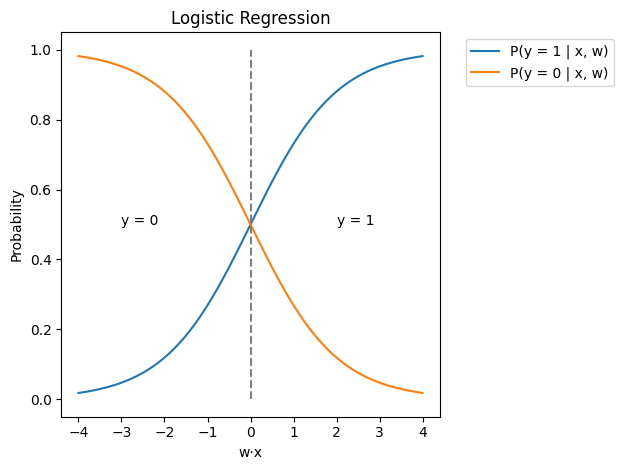
\includegraphics[scale=0.35]{images/05_01.png}
\end{center}

We then predict the label $\hat{y}$ as the label which has higher probability. Hence $\hat{y} = 1$ if:

\begin{align*}
           & \frac{P(y = 1 \pipe \tc{x}, \tc{w})}{P(y = 0 \pipe \tc{x}, \tc{w})} > 1 \\
  \implies & \frac{\sigma(\tc{w}^T\tc{x})}{1 - \sigma(\tc{w}^T\tc{x})} > 1           \\
  \implies & \exp(\tc{w}^T\tc{x}) > 1                                                \\
  \implies & \tc{w}^T\tc{x} > 0
\end{align*}

Hence, the \tc{hyperplane} $\tc{w}^T \tc{x} = 0$ acts as a \tc{decision boundary} in the sense that all input vectors $\tc{x}$ lying ``above'' the boundary (that is $\tc{w}^T \tc{x} > 0$) are given label $1$ and rest are given label $0$.

\begin{center}
  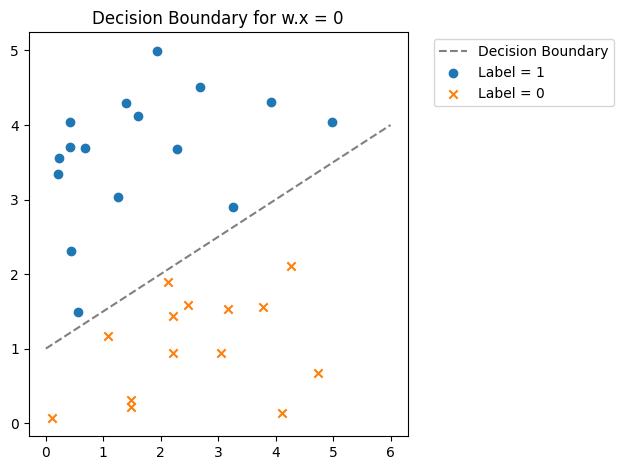
\includegraphics[scale=0.4]{images/05_02.png}
\end{center}

Observe that logistic regression yields a linear decision boundary. Hence it can perfectly classify the training points for \tc{linearly separable data}. \\

\fbox{
  \begin{minipage}{\textwidth}
    \tc{Linearly Separable Data}: A data-set $ \D$ is linearly separable if $\exists \tc{w}$ such that $\forall$ positive training points ($y = 1$), $\tc{w}^T\tc{x} > 0$ and $\forall$ negative training points ($y = 0$), $\tc{w}^T\tc{x} < 0$.
  \end{minipage}
} \\

This puts a severe restriction on the data-sets which can be classified using logistic regression. Consider a simple example, where $\tc{x} = [x_1, x_2]^T \in \mathbb{R}^2$ :

\begin{equation*}
  y = \begin{cases}
    1 \qq{if} x_1 \cdot x_2 > 0 \\
    0 \qq{otherwise}
  \end{cases}
\end{equation*}

\begin{center}
  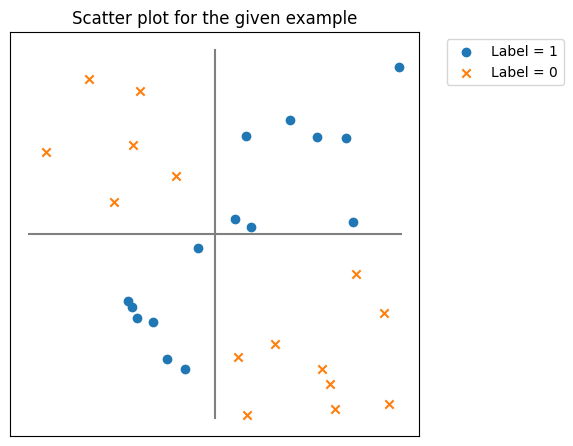
\includegraphics[scale=0.35]{images/05_03.png}
\end{center}

Observe that a Logistic Regression Classifier will not be able to find a good linear decision boundary for the above data. However, adding a feature to get $\phi(\tc{x}) = [1, x_1, x_2, x_1 x_2]^T$ makes the data linearly separable and enables the model to find a perfect weight vector $\tc{w} = [0, 0, 0, 1]^T$ to classify the data.

Hence, to get better results, we may have to add new features to the input vector before training the model.

\subsection{Parameter Estimation}

Since the output of model is a probability distribution on the labels, it is natural to estimate the parameters $\tc{w}$ as the \tc{Maximum Likelihood Estimate} for the observed data (training data-set). Hence,

\begin{align*}
  \tc{w}^* & = \underset{\tc{w}}{\text{argmax}} \prod_{i=1}^{| \D_{\text{train}}|} P(y_i | \tc{x}_i, \tc{w})                                           \\
           & = \underset{\tc{w}}{\text{argmax}} \sum_{i=1}^{| \D_{\text{train}}|} \log P(y_i | \tc{x}_i, \tc{w}) \qq{(Maximum Conditional Likelihood)} \\
           & = \underset{\tc{w}}{\text{argmin}}  \sum_{i=1}^{| \D_{\text{train}}|} -\log P(y_i | \tc{x}_i, \tc{w}) \qq{(Corresponding Loss Function)}
\end{align*}

Here, $ P(y_i \pipe \tc{x}_i, \tc{w}) $ is shorthand for $ P(\hat y_i = y_i\pipe \tc{x}_i, \tc{w}) $, where $P(\hat y_i = 1 \pipe \tc{x}_i, \tc{w}) = \sigma(\tc{w}^T \tc{x}_i)$.

Hence, the loss associated with a single data point is:

\begin{align*}
  L_{\tc{w}} (\tc{x}_i, y_i) = \begin{cases}
                                 -\log P(y_i = 1 \pipe \tc{x}_i, \tc{w}) \qq{if} y_i = 1 \\
                                 -\log (1 - P(y_i = 1 \pipe \tc{x}_i, \tc{w})) \qq{if} y_i = 0
                               \end{cases}
\end{align*}

Combining them,

\begin{equation*}
  \boxed{L (\tc{w}, \tc{x}_i, y_i) = -y_i \log P(y_i = 1 \pipe \tc{x}_i, \tc{w}) - (1 - y_i) \log (1 - P(y_i = 1 \pipe \tc{x}_i, \tc{w}))}
\end{equation*}

Total loss across the dataset then would be,

\begin{equation*}
  L  (\tc{w},  \D) = \sum_{i = 1}^{| \D|} \underbrace{-y_i \log P(y_i = 1 \pipe \tc{x}_i, \tc{w}) - (1 - y_i) \log (1 - P(y_i = 1 \pipe \tc{x}_i, \tc{w})) }_{\text{(Binary) Cross Entropy Loss}}
\end{equation*}

This loss is called the binary cross entropy loss because of the similar structure as the formula for cross-entropy loss in information theory. Some properties about the above defined cross entropy loss:

\begin{itemize}
  \item It is a convex loss function
  \item It is differentiable
  \item There is no closed form solution for the optimal parameter $\tc{w}^*$. Hence techniques such as gradient descent are used to optimise the model.
\end{itemize}

To calculate the gradient, note that \begin{align*}
  \nabla_{\tc{w}} \sigma(\tc{w}^T \tc{x}_i) & =  \sigma(\tc{w}^T \tc{x}_i)(1-\sigma(\tc{w}^T \tc{x}_i))\nabla_{\tc{w}} \tc{w}^T \tc{x}_i \\ &= \sigma(\tc{w}^T \tc{x}_i)(1-\sigma(\tc{w}^T \tc{x}_i))\tc{x}_i
\end{align*}
$$
  \implies \nabla_{\tc{w}} \log \sigma(\tc{w}^T \tc{x}_i) = (1-\sigma(\tc{w}^T \tc{x}_i))\tc{x}_i
$$
$$
  \nabla_{\tc{w}} \log (1 - \sigma(\tc{w}^T \tc{x}_i)) = -\sigma(\tc{w}^T \tc{x}_i)\tc{x}_i
$$
\begin{align*}
  \implies \nabla_{\tc{w}}L  (\tc{w},  \D) & =  \sum_{i = 1}^{| \D|}-y_i  (1-\sigma(\tc{w}^T \tc{x}_i))\tc{x}_i + (1 - y_i) \sigma(\tc{w}^T \tc{x}_i)\tc{x}_i \\&= \sum_{i = 1}^{| \D|}(\sigma(\tc{w}^T\tc{x}_i)-y_i) \tc{x}_i\\
                                           & = \sum_{i = 1}^{| \D|}(\hat y_i-y_i) \tc{x}_i
\end{align*}

The form of the gradient is very similar to that in linear regression, with $\hat y = \sigma(\tc{w}^T\tc{x}_i)$

This also shows convexity, since
\begin{align*}
  \nabla^2_{\tc{w}}L  (\tc{w},  \D) & = \nabla_{\tc{w}} \cdot \nabla_{\tc{w}} L (\tc{w},  \D)                                         \\
                                    & = \sum_{i = 1}^{|\D|} \nabla_{\tc{w}} \cdot (\sigma(\tc{w}^T\tc{x}_i)-y_i) \tc{x}_i             \\
                                    & = \sum_{i = 1}^{|\D|} \sigma(\tc{w}^T \tc{x}_i)(1-\sigma(\tc{w}^T \tc{x}_i)) \ ||\tc{x}_i||_2^2 \\
                                    & > 0
\end{align*}

and hence, gradient descent would be good option to minimise loss and find optimal paramters.

\section{Logistic Regression with Regularization}

Logistic regression is capable of perfectly classifying linearly separable data. But there may be mulitple weight vectors that can separate the data. Let us consider the case in which the dataset is linearly separable and the true decision boundary is represented by straight lines.

\begin{center}
  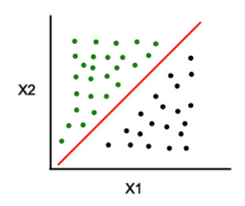
\includegraphics[scale=0.8]{images/05_04.png}
\end{center}

For the data given in the above diagram, the true decision boundary is represented by the straight line $x_1 - 2x_2 = 0$. However, the problem with the supposed values of $w_1 = 1, w_2 = -2$ is that they can be scaled up arbitrarily because the constant term is $0$. Hence, it raises the question as to what are the values of $\tc{w}$ that the logistic regression classifier is likely to converge at ? \\

We know that
$$
  \Pb(y_i = 1 \pipe \tc{x}_i, \tc{w}) = \sigma(\tc{w}^\top \tc{x}) = \frac{1}{1+\exp(-\tc{w}^\top \tc{x})}
$$

The aim of the classifier is to maximise the above probability for the points in the training dataset and thus it is likely that it will pump up the values of the weights to decrease the value of $\exp(-\tc{w}^Tw\tc{x})$ and thus increasing the value of $\Pb(y_i = 1 \pipe x_i,w)$ to about $1$ for all of the positive samples. Thus, in short it is likely that our classifier would choose high values of the weights $w$. \\

\tc{But is this ideal?}

\begin{center}
  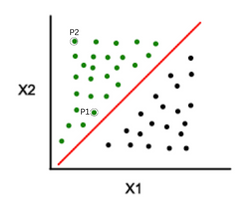
\includegraphics[scale=0.8]{images/05_05.png}
\end{center}

Consider two positive sample points as shown in the above figure, one very close to the decision boundary $P1$, and the other further away from the decision boundary $P2$. We would ideally want a higher value of
$$
  P(y_i = 1 \pipe \tc{x}_i,\tc{w}) = \sigma(\tc{w}^\top \tc{x}) = \frac{1}{1+\exp(-\tc{w}^\top\tc{x})}
$$

for $P2$ than $P1$ as it is far away from the decision boundary and thus confidence of prediction should be higher for this point than $P1$. Ideally, we want data points far from the decision boundary like $P2$ to have a higher probability of being correctly classified by the classifier, while data points near the decision boundary like $P1$ should not be excessively influenced and receive artificially higher probabilities of being classified into one of the regions. But when the values of the coefficients $w$ in logistic regression are arbitrarily high, it diminishes the distinction between data points located near the decision boundary and those far from it as the probability for all the positive samples nearly tends to 1. This occurs because the exponential term in the logistic function causes the probabilities assigned to both types of points to become substantially higher.  \\

To address this issue, we introduce a \tc{regularization term} along with the loss function.
$$
  \tc{w}^*_R = \arg\min_{\tc{w}} \ L_{CE}(\tc{w}, \D) + \lambda||\tc{w}||^2_2
$$

The regularization term's purpose is to impose constraints on the values of $\tc{w}$, preventing them from becoming arbitrarily high. By applying regularization, we effectively limit the coefficients' magnitudes, which helps maintain the proper distinction between data points and prevents the model from assigning overly confident probabilities to points near the decision boundary. \\

The regularization penalty term forces the model to find a balance between minimizing the cross entropy loss (fitting the data) and minimizing the regularization term (keeping coefficients small). This means that the model's predictions are less sensitive to minor fluctuations or noise in the training data. Consequently, the above model becomes more robust and less likely to overfit, leading to a \tc{reduction in variance}. \\

In logistic regression, when the decision boundary is linear, it is relatively straightforward to interpret the model. The feature interpretability of logistic regression models with linear decision boundaries is high which means we can easily assess the importance and relevance of each feature or attribute in making predictions. However, when dealing with non-linear decision boundaries, especially in models with numerous features, interpreting the model and selecting the most informative features becomes much more challenging. \\

There are 2 desired features of classification models:
\begin{enumerate}
  \item The ability to learn complex decision boundaries.
  \item Interpretability of the model i.e. how useful are each of the features/attributes.
\end{enumerate}

Non-linear logistic regression models aren't easily interpretable and so now, we move onto another kind of classifiers which are Decision Tree Classifiers.

\section{Decision Trees: Learning complex decision boundary}
Decision tree is an interpretable model whose final prediction can be written as a \tc{disjunction of conjunctions} based on the attribute values over training instances.

\begin{center}
  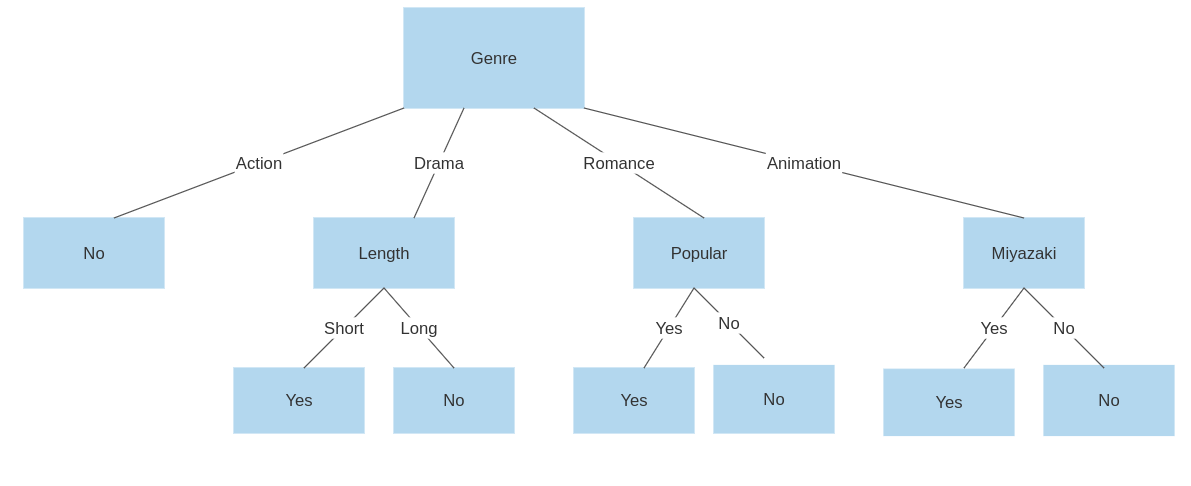
\includegraphics[width=\textwidth]{images/05_06.png}
\end{center}

The above figure is an example of a decision tree. It represets how decisions might be made by a decision tree to classify movies that are liked (represented by 'Yes') or disliked (represented by 'No') by a person. Each node of the tree represents an attribute and each path of the tree represents a conjuction of attributes and the final decision is a disjunction of these conjuctions. For instance for the above tree, the final prediction of the model can be written as
\begin{align*}
   & (Genre = Drama \ \wedge \ Length = Short) \vee (Genre = Romance \ \wedge \ Popular = Yes) \\
   & \vee (Genre = Animation \ \wedge \ Mizayaki = Yes)
\end{align*}

The above expression evaluates to true (yields the value 1) for a 'Yes' instance and evaluates to false (yields the value 0) for a 'No' instance.

\subsection{Decision Boundaries of Decision Trees}
Consider the following xor-like classified dataset

\begin{center}
  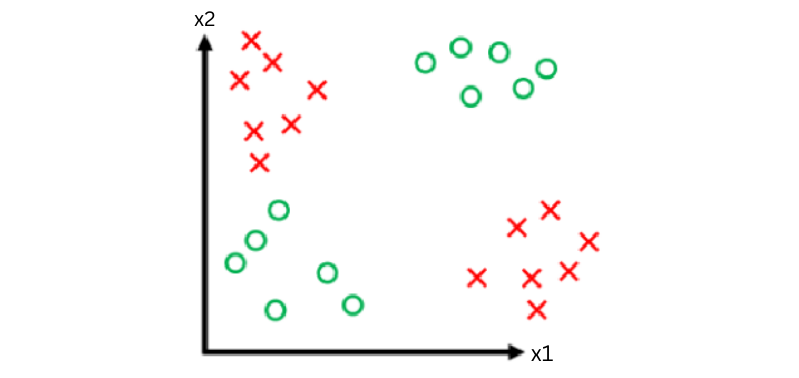
\includegraphics[width=0.8\textwidth]{images/05_07.png}
\end{center}

The x and y axis correspond to 2 attributes of the dataset, $x1$ and $x2$ respectively. The datapoints marked by green circles and the datapoints marked by red crosses represent 2 different categories $(y_{labels})$ say category 1 and category 2 respectively. \\

The following might be the decision tree for the classification of the above dataset.
\begin{center}
  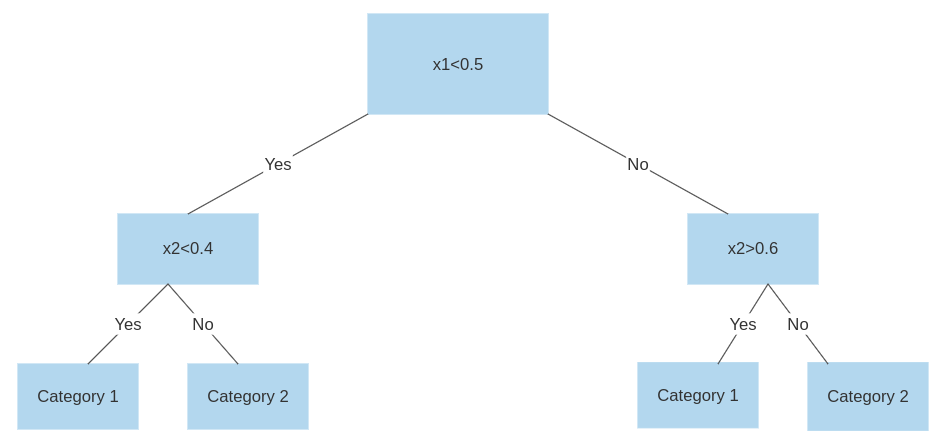
\includegraphics[width=\textwidth]{images/05_08.png}
\end{center}

If the condition in the topmost decision node of the decision tree that is $x_{1} < 0.5$ evaluates to true, we move along the left edge of the tree and right otherwise. After traversing an edge, we either land on the condition(node) $x_{2} < 0.4$ or $x_{2} > 0.6$ respectively. If the condition in the node evaluates to true, we move along the left edge and we move along the right edge in case the condition evaluates to false. If we have moved along the left edge, in this example decision tree, we predict category 1(represented by green circles) or else we predict category 2(represented by red crosses) \\

Thus, on the basis of the above decision tree, the decision boundaries of the decision tree are as follows:
\begin{center}
  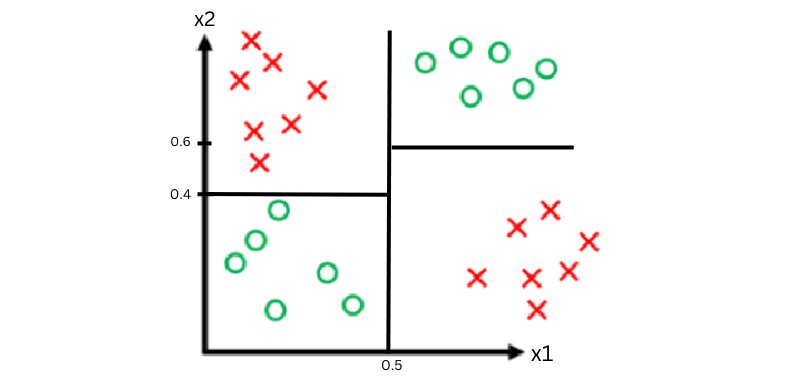
\includegraphics[width=0.8\textwidth]{images/05_09.png}
\end{center}

The vertical line represents the topmost decision node of the decision tree that is $x_{1} < 0.5$ and the two horizontal lines represent $x_{2} < 0.4$ and $x_{2} > 0.6$ respectively. We can see that the decision boundaries are just the depiction of the nodes (the attributes based on which decisions were taken) of the decision tree when plotted on a graph. \\

Thus, as seen above if nodes of the decision tree depend on a single attribute only, then decision trees divide the feature space into \tc{hyper-rectangles} or equivalently we can say that the resulting decision boundaries are axis-parallel hyper-planes.

\begin{mdframed}
  \tc{NOTE}: Instead of axis-parallel hyperplanes, we can even have linear hyper-planes. In the later case, instead of the decision nodes being a linear function of a single attribute, they can be a linear function of 2 or more attributes, say for instance $x_{1} + x_{2}>0$. Thus, in such cases instead of axis-parrallel decision boundaries, we would have locally-linear decision boundaries.
  Typically, axis-parallel hyperplanes are used for decision tree modelling.
\end{mdframed}

\subsection{Finding the optimal Decision Tree}
Unlike the case for logistic regression, finding the smallest Decision Tree that is optimal with respect to some metric (like cross entropy loss etc.) involving all of the attributes is an \tc{NP-hard problem}.

Decision tree estimation is done rather largely \tc{greedily} in which the tree is built recursively.

\vspace{2 mm}

Here's a simple decision tree template:
\begin{itemize}
  \setlength\itemsep{0pt}
  \item Start from an empty node with all instances.
  \item Pick the \tc{best} attribute to split on. For instance in figure 1, genre was chosen as the first attribute
  \item Repeat step 2 recursively for each new node until a \tc{stopping criterion} is met
\end{itemize}
\vspace{2mm}

Now, two important questions arise:
\begin{itemize}
  \setlength\itemsep{0pt}
  \item What is the notion of best attribute and how do we find it?
  \item What is a good stopping criterion?
\end{itemize}
\vspace{2mm}

It is to be noted that a lot of heuristics are involved in decision tree construction which is different from logistic regression we have studied in which we had a clearly formulated optimisation problem and a final solution to the optimisation problem. \\

We will start by reflecting on how to choose the best attribute.

\subsection{Choosing node attributes}

\begin{center}
  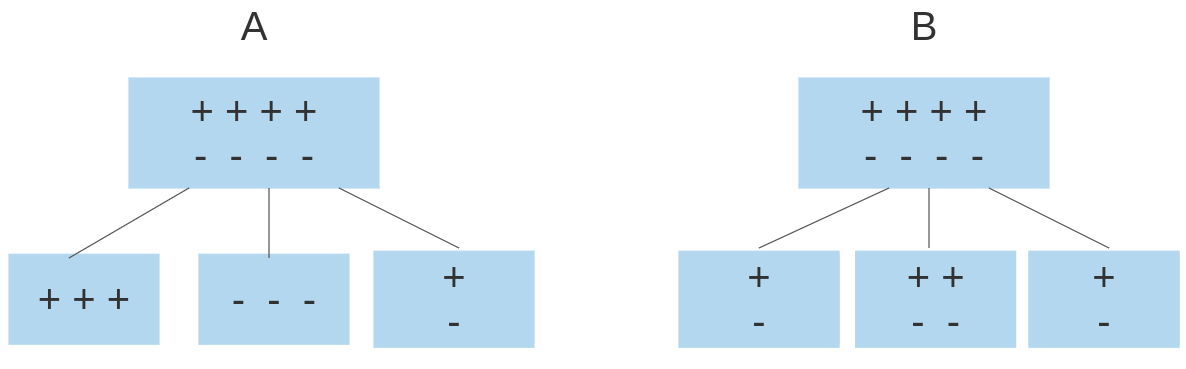
\includegraphics[width=\textwidth]{images/05_10.png}
\end{center}

Unlike the previous trees we have seen, the nodes of the above tree represent the datapoints that would reach these nodes based on the values of some attribute. In both of the above images, the topmost node represents the entire dataset (as no division of the dataset on the basis of some attribute has been done yet). Then on the basis of some attribute which is clearly different for $A$ and $B$, the dataset is divided into 3 datasets which are present in the three child nodes of each parent. \\

Seeing the above classification, it seems intuitive that the attribute on which decision has been taken in $A$ is better than the one in $B$. This is because, $A$'s attribute is leading to nodes that are already largely \tc{homogeneous} and thus the attribute in $A$ immediately effectively reduces the length of the decision tree. \\

On extending the tree, $B$ might later on have better accuracy but the top attribute is just overly building out the tree which is not preferable as overly large trees might lead to overfitting. Thus, our goal somewhat broadly is find simple models that generate good subtrees that get added on and we want the size of subtrees to be as small as possible. \\

\begin{mdframed}
  \tc{Intuition for a good split (attribute)}: A good split for an attribute results in subsets that are (mostly) entirely homogeneous that is the dataset in each split is (mostly) all of the same category.
\end{mdframed}

Now, we need a quantitative way to suit our intuitions for a good attribute and thus we introduce the following concepts.

\subsection{Entropy}

Entropy of a random variable is a measure of \tc{uncertainty} in the value of that random variable. Let $X$ be a random variable and $x$ represent a particular value of the random variable. Entropy  of X is H(X) where H(X) is defined as
$$
  H(X) =  -\sum_{x} \Pb(X=x)\log_{2} (\Pb(X=x))
$$

To understand what $H(X)$ signifies, let's pick up our familiar coin toss example in which the random variable can take the value 1 or 0 on the basis of the result of the coin toss (heads or tails respectively). $H(X)$ for this random variable is plotted below:

\begin{figure}[H]
  \centering
  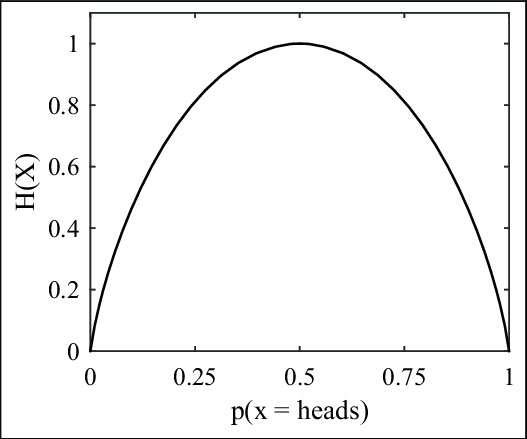
\includegraphics[width=0.4\textwidth]{images/05_11.png}
  \caption{Entropy of a coin toss}
\end{figure}

If the coin is fair (P(Head) = P(Tail) = 0.5) then there is maximum uncertainty in  toss outcome and thus entropy has a maxima at this point and if the coin is heavily biased (e.g P(Head)= 0.9, P(Tail)= 0.1) then there is some certainty about whether it would be head or tail and thus entropy is low. Thus, higher the uncertainty in the outcome of the random variable, higher is the entropy.
Thus it can be said that,
\begin{itemize}
  \item A high value of entropy asserts a nearly uniform distribution . We do not know the next outcome(e.g coin toss).
  \item A lower value of Entropy asserts that the distribution of the random variable has well-defined modes and thus there is some certainty in the outcome of the random variable.
\end{itemize}

\subsection{Entropy of a Dataset}

Entropy of a dataset measures the uncertainty in the group of observations. Consider a dataset $S$ with k classes/labels. Entropy of the dataset $S$ is $H(S)$ where $H(S)$ is defined as
$$
  H(S) =  -\sum_{i=1}^{k} \Pb_{i,S}\log (\Pb_{i,S})
$$

where $\Pb_{i,S}$ is the relative count of instances in $S$ with label i (the probability of randomly selecting an example of class i in $S$).\\
What happens when all instances belong to the same class? $\Pb_{i,s}$ is 1 which implies that entropy of the dataset is 0. \\

\fbox{
  \begin{minipage}{\textwidth}{
      \tc{Entropy} The entropy defined above is conceptually very similar to that in physics and chemistry. Remember this (from JEE days)?
      $$\Delta S_\text{mix} = -R(n_1+n_2)\bigg(\frac{n_1}{n_1+n_2}\ln \frac{n_1}{n_1+n_2} + \frac{n_2}{n_1+n_2}\ln \frac{n_2}{n_1+n_2}\bigg)$$
      Its the entropy of mixing 2 gases ($n_1$ and $n_2$ mols). Apart from the multiplicative constants, the expression is the same as $H(S)$.
    }
  \end{minipage}
}

\section{Information Gain}

Finding the optimal way of splitting the data is NP-hard. So we resort to using heuristic greedy strategies to get a reasonably good split. \\

\fbox{
  \begin{minipage}{\textwidth}
    \tc{Heuristic} is a technique designed for problem solving more quickly when classic methods are too slow for finding an exact or approximate solution, or when classic methods fail to find any exact solution. This is achieved by trading optimality, completeness, accuracy, or precision for speed. In a way, it can be considered a shortcut.
  \end{minipage}
}
\vspace{3mm}

One common heuristic measure used in the context of decision trees is the \tc{information gain}. \\

Suppose we now we choose an attribute $a$ from one of $x_1,\dots,x_n$. Suppose $a$ can attain values from $\text{Values}(a)$. All the elements of $s \in S$ which have $\gamma$ as the value of attribute $a$ will be placed in $S_\gamma$. Now, the information gain is defined as
$$
  \text{Gain}(S,a) = H(S) - \sum_{\gamma\in \text{Values}(a)}\frac{|S_\gamma|}{|S|}H(S_\gamma)
$$

\tc{Intuition} : suppose we choose an ideal attribute that separates all the labels perfectly, then each of $H(S_\gamma)$ will be zero and information gain will be maximum. To gain information we need to reduce entropy by separating the elements. The factor $\frac{|S_\gamma|}{|S|}$ is needed to account for the fact that the set sizes are different.

The attribute that gives the maximum information gain is the best attribute to split.
$$a^* = \argmax_{a} \text{Gain}(S,a)$$
Apart from information gain there are other heuristics like \tc{Gini impurity} that are commonly used in DTs. \\

\fbox{
  \begin{minipage}{\textwidth}{
      \tc{Information Theory Basis} \\

      The information gain that we defined above is called as \tc{mutual information} in information theory.
      $$
        I(X,Y) = H(Y) - H(Y|X) = H(X) - H(X|Y)
      $$
      where $H(X|Y)$ is the conditional entropy.
      $$
        H(X|Y) = \sum_i p(X = x_i) H(Y|X = x_i)
      $$
    }
  \end{minipage}
}
\vspace{4mm}

\tc{Example}: Consider a dataset (Table 1) with two boolean attributes $x_1$ and $x_2$ and label $y$. Let us find the optimal attribute to split.

\begin{table}[ht]
  \centering
  \begin{tabular}{|c|c|c|}
    \hline
    $x_1$ & $x_2$ & $y$ \\
    \hline
    1     & 1     & 1   \\
    \hline
    1     & 0     & 1   \\
    \hline
    1     & 1     & 1   \\
    \hline
    1     & 0     & 1   \\
    \hline
    0     & 1     & 1   \\
    \hline
    0     & 0     & 0   \\
    \hline
  \end{tabular}
  \caption{Dataset for the example}
\end{table}

$$
  H(S) = -\bigg(\frac{5}{6}\log_2 \frac{5}{6} + \frac{1}{6}\log_2 \frac{1}{6} \bigg) = 0.65
$$
$$
  \text{Gain}(S,x_1) = H(S) - \bigg( \frac{4}{6} \times 0 + \frac{2}{6}\times1\bigg) = 0.32
$$
$$
  \text{Gain}(S,x_2) = H(S) - \bigg( \frac{3}{6} \times 0 + \frac{3}{6}\times0.92\bigg) = 0.19
$$

Since information gain is maximum when split using $x_1$, it is best to split using $x_1$.
\vspace{8mm}

Till now we have considered the attributes of dataset to be discrete variables. What if they are continuous? In case of discrete attribute we can easily split using the different values of the attribute. For \tc{continuous} attributes, we need to identify thresholds ($\tau$) for the attribute values that we can use to design binary questions of the kind, ``Is attribute $a \le \tau$?" with yes/no answers. Here is the procedure to identify these thresholds:
\begin{itemize}
  \item Let $v_1,\dots,v_n$ be the values of attribute $a$ in the training set.
  \item Sort the values in increasing order : $v_{i_1},\dots,v_{i_n}$.
  \item Midpoint $m_j$ is defined as
        $$m_j = \frac{v_{i_j} + v_{i_{j+1}}}{2}$$
  \item Choose all such midpoints $m_j$ whose underlying instances on either side have different labels. These midpoints will serve as thresholds for this continuous attribute.
\end{itemize}

For example, consider an attribute $a$ that takes the values $\{10, 26, 40, 50, 100, 120\}$ across six training instances with corresponding labels $\{0, 0, 0, 1, 1, 0\}$. The midpoints are $\{18, 33, 45, 75, 110\}$, and the ones that will get picked up as thresholds are $\{45, 110\}$ since they are midpoints located between two instances with differing labels. Thus, the questions that can be asked relevant to attribute $a$ are ``Is $a \le 45$?" and ``Is $a > 110?$". \\

\tc{Example:} Consider the dataset in Table 2 with two attributes $x_1,x_2$ which are real numbers. Each instance of the dataset has an associated binary label $y$ ($0$ or $1$).

\begin{table}[ht]
  \centering
  \begin{tabular}{|c|c|c|}
    \hline
    $x_1$ & $x_2$ & $y$ \\
    \hline
    0.1   & 0.53  & 1   \\
    \hline
    0.2   & 0.86  & 1   \\
    \hline
    0.25  & 0.36  & 0   \\
    \hline
    0.36  & 0.91  & 1   \\
    \hline
    0.47  & 0.87  & 1   \\
    \hline
    0.65  & 0.13  & 0   \\
    \hline
    0.71  & 0.82  & 0   \\
    \hline
    0.85  & 0.55  & 0   \\
    \hline
  \end{tabular}
  \caption{Dataset for the example}
  \label{tab:my_label}
\end{table}

Let us start by splitting using $x_1$. (See the figure below)
\begin{figure}[ht]
  \centering
  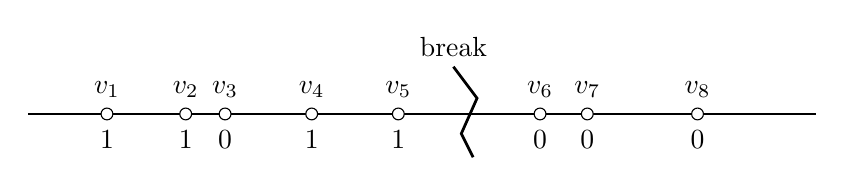
\begin{tikzpicture}[
      M/.style={draw, minimum size = 0.15cm, fill = white, shape = circle, inner sep=0pt}
    ]
    \draw (0,0) -- (10,0);
    \draw (1,0) node [M, label=north:$v_1$, label=south:$1$] {};
    \draw (2,0) node [M, label=north:$v_2$, label=south:$1$] {};
    \draw (2.5,0) node [M, label=north:$v_3$, label=south:$0$] {};
    \draw (3.6,0) node [M, label=north:$v_4$, label=south:$1$] {};
    \draw (4.7,0) node [M, label=north:$v_5$, label=south:$1$] {};
    \draw (6.5,0) node [M, label=north:$v_6$, label=south:$0$] {};
    \draw (7.1,0) node [M, label=north:$v_7$, label=south:$0$] {};
    \draw (8.5,0) node [M, label=north:$v_8$, label=south:$0$] {};
    \draw [line width = 1pt] (5.4, 0.6) node [anchor = south] {break} -- (5.7,0.2) -- (5.5,-0.25) -- (5.65,-0.55);
  \end{tikzpicture}
  \caption{Visualisation of attribute $x_1$ of Table 2}
  \label{fig:enter-label}
\end{figure}

To maximise information gain, we split between $v_5$ and $v_6$ using
$$m_5 = \frac{v_5+v_6}{2} = 0.56$$

\section{Stopping Criteria}
Now we come to the second question, when do we stop splitting?  These are some of the stopping criteria that help avoid overfitting to the data.
\begin{itemize}
  \item Stop splitting if all the instances have the same label.
  \item Do not split if the number of instances at a node is less than $k$ ($k$ is some constant).
  \item Do not split if the number of leaf nodes exceed a certain threshold.
  \item Do not split if information gain at a node is below a certain threshold.
\end{itemize}
The above criteria act as some form of regularization for the DTs. Limiting the max depth of the tree is another possible regularization.

\section{Pruning}
This is an alternate approach to tackle overfitting. Here we build the complete tree and then remove/prune some of the non-critical/redundant branches. To evaluate the performance after pruning, validation set is used.

Pruning a node means replacing the subtree rooted at the node with a leaf node whose label is the max label of the node that was pruned. We can use a greedy approach to pruning:
\begin{enumerate}
  \item Pick a node which when pruned results in the highest gain in validation accuracy.
  \item Repeat step 1 until there is no further improvement in validation accuracy.
\end{enumerate}
This is called as \tc{reduced error pruning}.

\section{Random Forests (Brief Introduction)}

Decision trees in the form that we studied till now, are very rarely used today. However, DTs are used in random forests (RTs), which is a very common method in \tc{ensemble} learning. An ensemble method uses a combination of methods/models to predict the final output. A random forest is an ensemble model which uses \tc{bootstrap aggregation} or \tc{bagging}. \\

Bagging involves training an ensemble on bootstrapped data sets. Consider a dataset $\mathcal{D}$ having $n$ samples in it (that is $|\mathcal{D}| = n$). Now we generate $m$ datasets $\mathcal{D}_1,\dots,\mathcal{D}_m$ each of the same size $n$ ($|\mathcal{D}_1| = \dots = |\mathcal{D}_m| = n$) by randomly sampling (with replacement) from $\mathcal{D}$. As a result an instance  $d \in \mathcal{D}$ might occur zero, once or more than once in $\mathcal{D}_i$. Each of the $m$ datasets is used in training a separate model. The final prediction is made by \tc{aggregating} the results of each of the models (example averaging or voting). \\

Random forests are bagged DTs, each of the $m$ datasets is made into a separate DT. In each of these DTs, we pick a random set $S$ (not too small not too large) of attributes to split the data. Taking very small set of attributes will result in losing too much information and taking too many will result in all the $m$ models being nearly the same. \\

\begin{figure}[H]
  \centering
  \begin{subfigure}[t]{0.45\textwidth}
    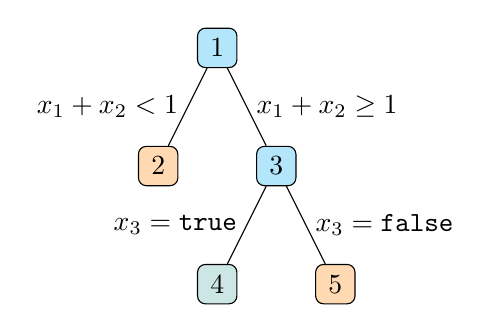
\begin{tikzpicture}[
        M/.style={draw, rounded corners=.1cm, minimum size=0.5cm, fill = cyan!30}
      ]
      \node [M] {1}
      child {node[M, fill = orange!30] {2}
          edge from parent node [left] {$x_1+x_2 < 1$}}
      child {node[M] {3}
          child {node[M, fill = teal!20] {4}
              edge from parent node [left] {$x_3 = \texttt{true}$}}
          child {node[M, fill = orange!30] {5}
              edge from parent node [right] {$x_3 = \texttt{false}$}}
          edge from parent node [right] {$x_1+x_2 \geq 1$}};
    \end{tikzpicture}
    \caption{Tree 1}
  \end{subfigure}
  \begin{subfigure}[t]{0.45\textwidth}
    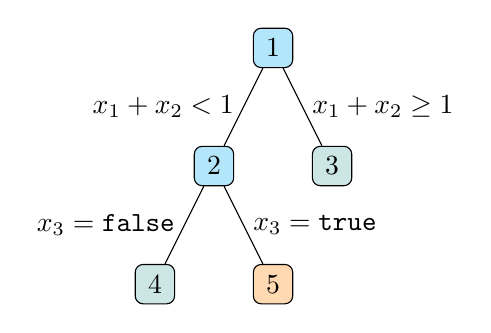
\begin{tikzpicture}[
        M/.style={draw, rounded corners=.1cm, minimum size=0.5cm, fill = cyan!30}
      ]
      \node [M] {1}
      child {node[M] {2}
          child {node[M, fill = teal!20] {4}
              edge from parent node [left] {$x_3 = \texttt{false}$}}
          child {node[M, fill = orange!30] {5}
              edge from parent node [right] {$x_3 = \texttt{true}$}}
          edge from parent node [left] {$x_1+x_2 < 1$}}
      child {node[M, fill = teal!20] {3}
          edge from parent node [right] {$x_1+x_2 \geq 1$}};
    \end{tikzpicture}
    \caption{Tree 2}
  \end{subfigure}
  \caption{A random forest with $m = 2$}
\end{figure}